\section{Vorgehensmodelle}
\subsection{Phasenmodell - Wasserfall-Model}
Es ist einfach, klare Struktur. Jede Phase erzeugt ein Ergebnis, auf dem die nächste Phase aufbaut. Bekannte Vertreter sind Wasserfall oder V-Modell. Jedoch werden Planungsfehler erst spät bemerkt. Risiken werden zu spät erkannt. 
\subsubsection{Wasserfallmodell}
\begin{center}
	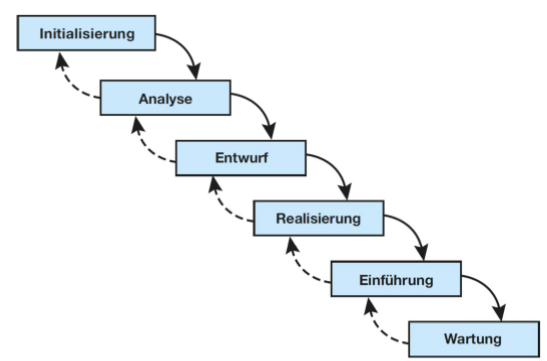
\includegraphics[width=0.6\columnwidth]{Images/Wasserfallmodell}
\end{center}

\subsubsection{V-Modell}
Starke Einbindung der Tests zu jeder Phase. Ähnlich wie bei Wasserfallmodell, auch hier ist eine grosse Erfahrung nötig
\begin{center}
	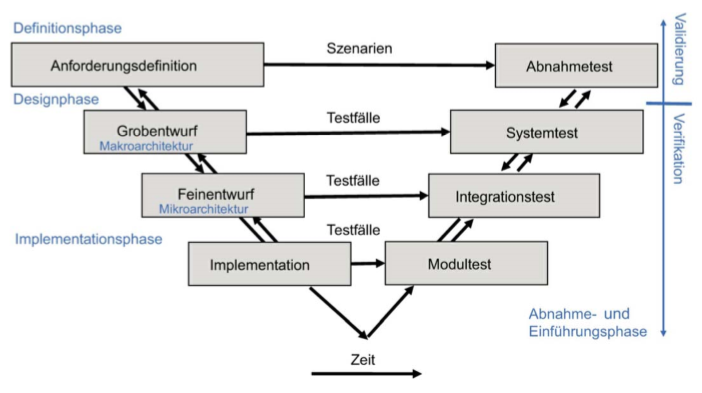
\includegraphics[width=0.6\columnwidth]{Images/v-modell}
\end{center}


\subsection{Agile}
Agile bedeutet "flink, beweglich". Ziel von der Agilen Softwareentwicklung ist es, eine leichtgewichtigen Ansatz mit hoher Flexibilität zu gewährleisten zB um Änderungen gut und schnell aufnehmen zu können ohne weitere Probleme. Agile Projekte werden vorallem für Software-Projekte eingesetzt, da Software-Entwicklung sehr flexibel ist. Für grosse und langlebige Projekte mit zB Regolatorischen-Anforderungen nicht geeignet (tailoring Notwendig aka. \textbf{Hybrid-Modell}).

\subsubsection{Spiralenmodell}
Ein iterativer/inkrementeller Vorgehen. Erlaubt kontinuerliche Lernkurven und eine schnelles Feedback vom Kunden. Ergebnisse der Zyklen wie Anforderung oder Architektur werden bei jeder Iteration verfeinert und Risiken frühzeitig erkannt.
\begin{center}
	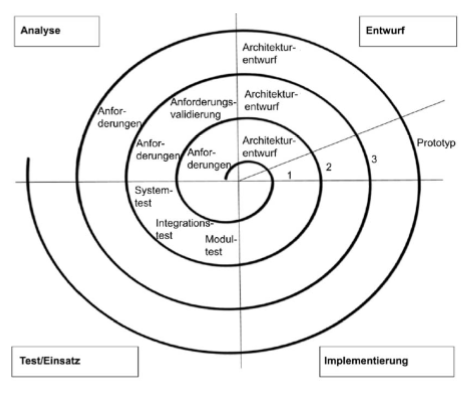
\includegraphics[width=0.6\columnwidth]{Images/spiralmodell}
\end{center}

\subsubsection{Scrum}
Ein agiles und sehr bekanntes Vorgehensmodel ist Scrum. Es werden dabei grob in drei Phasen unterteilt:
\begin{enumerate}[nosep]
	\item Grobplanung: Allgemeine Ziele festlegen und Software-Architektur planen
	\item Inkrementelles Entwicklung der Software
	\item Projektabschluss, Dokumentation werden vervollständigt und Lehren aus dem Projekt werden gezogen.
\end{enumerate}

In Scrum sind folgende Keywords unabdingbar:\\
\begin{tabular}{lm{6cm}}
	\textbf{Backlog} & Eine art To-Do Liste (Ansammlung von UserStories) die das Scrum-Team abarbeitet muss. \\
	\textbf{User Story} & Beschreiben Aufgaben, welche vom System gefordert werden. Sie müssen nicht von Anfang an detailiert sein, müssen aber bei der Umsetzung genau spezifiziert sein. \\
	\textbf{Product Owner} & Ein Kunde oder auch Projektmanager. Definiert was das Produkt können muss \\
	\textbf{Sprint} & Eine Entwicklungsiteration, Dauer in der Regel zwischen 2-4 Wochen. Definiert welche UserStories in der Itaration umgesetzt werden (Diese UserStories dürfen nicht mehr geändert werden) \\
	\textbf{Scrum} & Tägliches Meeting des Scrum-Teams, bei dem Fortschritt, Probleme und priorität überprüft werden.\\
	\textbf{Scrum Master} & Stellt sicher, dass Scrum-Prozess eingehalten wird. Er ist nicht der Projektleiter! \\
	\textbf{Velocity} & Eine Schätzung, wie viel vom Backlog ein Team in einem Sprint abdecken kann. Bietet eine Messung für die Leistungsbewertung des Teams.
\end{tabular}

\subsection{Hybrid-Modell}
Keine Modell ist perfekt, in der Praxis werden daher die Vorgehensmodelle vermischt und je nach Firma unterschiedliche angewandt. Im folgenden ein Beispiel
\begin{center}
	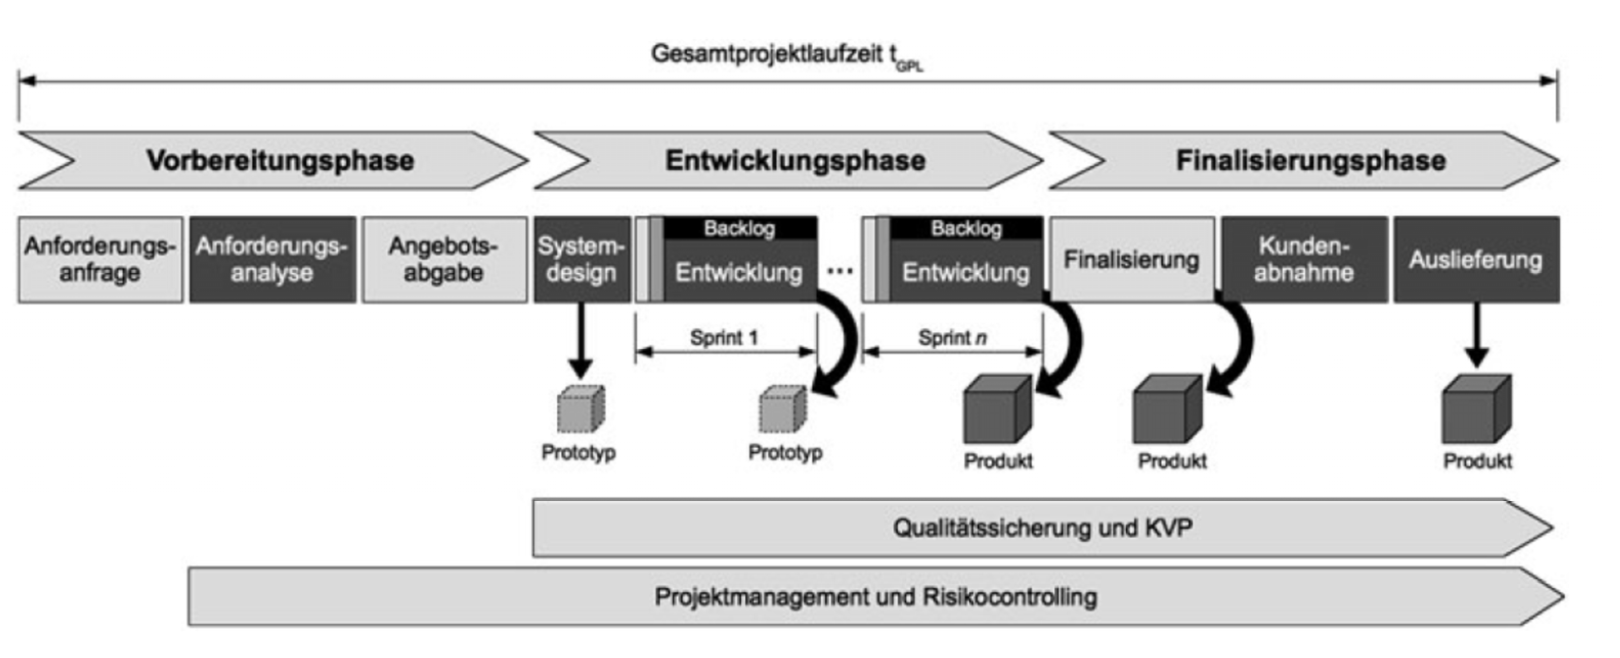
\includegraphics[width=\columnwidth]{Images/vorgehensmodell_beispiel}
\end{center}
